\ifx\allfiles\undefined
\documentclass[12pt, a4paper,oneside, UTF8]{ctexbook}
\usepackage[dvipsnames]{xcolor}
\usepackage{amsmath}   % 数学公式
\usepackage{amsthm}    % 定理环境
\usepackage{amssymb}   % 更多公式符号
\usepackage{graphicx}  % 插图
%\usepackage{mathrsfs}  % 数学字体
%\usepackage{newtxtext,newtxmath}
%\usepackage{arev}
\usepackage{kmath,kerkis}
\usepackage{newtxtext}
\usepackage{bbm}
\usepackage{enumitem}  % 列表
\usepackage{geometry}  % 页面调整
%\usepackage{unicode-math}
\usepackage[colorlinks,linkcolor=black]{hyperref}

\usepackage{wrapfig}


\usepackage{ulem}	   % 用于更多的下划线格式,
					   % \uline{}下划线,\uuline{}双下划线,\uwave{}下划波浪线,\sout{}中间删除线,\xout{}斜删除线
					   % \dashuline{}下划虚线,\dotuline{}文字底部加点


\graphicspath{ {flg/},{../flg/}, {config/}, {../config/} }  % 配置图形文件检索目录
\linespread{1.5} % 行高

% 页码设置
\geometry{top=25.4mm,bottom=25.4mm,left=20mm,right=20mm,headheight=2.17cm,headsep=4mm,footskip=12mm}

% 设置列表环境的上下间距
\setenumerate[1]{itemsep=5pt,partopsep=0pt,parsep=\parskip,topsep=5pt}
\setitemize[1]{itemsep=5pt,partopsep=0pt,parsep=\parskip,topsep=5pt}
\setdescription{itemsep=5pt,partopsep=0pt,parsep=\parskip,topsep=5pt}

% 定理环境
% ########## 定理环境 start ####################################
\theoremstyle{definition}
\newtheorem{defn}{\indent 定义}[section]

\newtheorem{lemma}{\indent 引理}[section]    % 引理 定理 推论 准则 共用一个编号计数
\newtheorem{thm}[lemma]{\indent 定理}
\newtheorem{corollary}[lemma]{\indent 推论}
\newtheorem{criterion}[lemma]{\indent 准则}

\newtheorem{proposition}{\indent 命题}[section]
\newtheorem{example}{\indent \color{SeaGreen}{例}}[section] % 绿色文字的 例 ,不需要就去除\color{SeaGreen}{}
\newtheorem*{rmk}{\indent \color{red}{注}}

% 两种方式定义中文的 证明 和 解 的环境:
% 缺点:\qedhere 命令将会失效【技术有限,暂时无法解决】
\renewenvironment{proof}{\par\textbf{证明.}\;}{\qed\par}
\newenvironment{solution}{\par{\textbf{解.}}\;}{\qed\par}

% 缺点:\bf 是过时命令,可以用 textb f等替代,但编译会有关于字体的警告,不过不影响使用【技术有限,暂时无法解决】
%\renewcommand{\proofname}{\indent\bf 证明}
%\newenvironment{solution}{\begin{proof}[\indent\bf 解]}{\end{proof}}
% ######### 定理环境 end  #####################################

% ↓↓↓↓↓↓↓↓↓↓↓↓↓↓↓↓↓ 以下是自定义的命令  ↓↓↓↓↓↓↓↓↓↓↓↓↓↓↓↓

% 用于调整表格的高度  使用 \hline\xrowht{25pt}
\newcommand{\xrowht}[2][0]{\addstackgap[.5\dimexpr#2\relax]{\vphantom{#1}}}

% 表格环境内长内容换行
\newcommand{\tabincell}[2]{\begin{tabular}{@{}#1@{}}#2\end{tabular}}

% 使用\linespread{1.5} 之后 cases 环境的行高也会改变,重新定义一个 ca 环境可以自动控制 cases 环境行高
\newenvironment{ca}[1][1]{\linespread{#1} \selectfont \begin{cases}}{\end{cases}}
% 和上面一样
\newenvironment{vx}[1][1]{\linespread{#1} \selectfont \begin{vmatrix}}{\end{vmatrix}}

\def\d{\textup{d}} % 直立体 d 用于微分符号 dx
\def\R{\mathbb{R}} % 实数域
\def\N{\mathbb{N}} % 自然数域
\def\C{\mathbb{C}} % 复数域
\def\Z{\mathbb{Z}} % 整数环
\def\Q{\mathbb{Q}} % 有理数域
\newcommand{\bs}[1]{\boldsymbol{#1}}    % 加粗,常用于向量
\newcommand{\ora}[1]{\overrightarrow{#1}} % 向量

% 数学 平行 符号
\newcommand{\pll}{\kern 0.56em/\kern -0.8em /\kern 0.56em}

% 用于空行\myspace{1} 表示空一行 填 2 表示空两行  
\newcommand{\myspace}[1]{\par\vspace{#1\baselineskip}}

%s.t. 用\st就能打出s.t.
\DeclareMathOperator{\st}{s.t.}

%罗马数字 \rmnum{}是小写罗马数字, \Rmnum{}是大写罗马数字
\makeatletter
\newcommand{\rmnum}[1]{\romannumeral #1}
\newcommand{\Rmnum}[1]{\expandafter@slowromancap\romannumeral #1@}
\makeatother
\begin{document}
	% \title{{\Huge{\textbf{$Real \,\, Analysis$}}}\\
		\Large{\textbf{$Measure \,\, Theory , \,\, Integration , \,\, \& \,\, Hilbert \,\, Spaces$}}\footnote{参考书籍:\\
			\hspace*{4em} \textbf{《$Real \,\, Analysis -- Measure \,\, Theroy, \,\, Integration, \,\, \& \,\, Hilbert \,\, Spaces$》--- $Elias \,\, M. \,\, Stein$} \\
			\hspace*{4em} \textbf{《$Real \,\, Analysis -- Modern \,\, Techniques \,\, and \,\, Their \,\, Applications$》--- $Gerald \,\, B. \,\, Folland$}}}
\author{$-TW-$}
\date{\today}
\maketitle                   % 在单独的标题页上生成一个标题

\thispagestyle{empty}        % 前言页面不使用页码
\begin{center}
	\Huge\textbf{序}
\end{center}


\vspace*{3em}
\begin{center}
	\large{\textbf{天道几何,万品流形先自守;}}\\
	
	\large{\textbf{变分无限,孤心测度有同伦。}}
\end{center}

\vspace*{3em}
\begin{flushright}
	\begin{tabular}{c}
		\today \\ \small{\textbf{长夜伴浪破晓梦,梦晓破浪伴夜长}}
	\end{tabular}
\end{flushright}


\newpage                      % 新的一页
\pagestyle{plain}             % 设置页眉和页脚的排版方式(plain:页眉是空的,页脚只包含一个居中的页码)
\setcounter{page}{1}          % 重新定义页码从第一页开始
\pagenumbering{Roman}         % 使用大写的罗马数字作为页码
\tableofcontents              % 生成目录

\newpage                      % 以下是正文
\pagestyle{plain}
\setcounter{page}{1}          % 使用阿拉伯数字作为页码
\pagenumbering{arabic}
\setcounter{chapter}{0}    % 设置 -1 可作为第零章绪论从第零章开始 
	\else
	\fi
	%  ############################ 正文部分
\appendix

\chapter{命题证明}
\setcounter{section}{4}

\section{$\S 1.5$}
	\begin{enumerate}
		\item \textbf{Prop \ref{prop 2.5.1}. 半区间基本集族生成代数上的预测度}. \\
		\begin{proof}
			首先证明$\mu_0$ 是良定义的,此处省略 (比较Trivial). \\
			下面证明$\mu_0$ is a premeasure on algebra $\mathcal{A}$. \\
			Suppose $\{ A_j \}_{j = 1}^{\infty} \subset \mathcal{A}$ disjoint with $\overset{\infty}{\underset{j = 1}{\bigcup}}{A_j} \in \mathcal{A}$. WTS
			\begin{align}
				\mu_0(\bigcup_{j = 1}^{\infty}{A_j}) = \sum_{j = 1}^{\infty}{\mu_0(A_j)}
			\end{align}
			Since $\overset{\infty}{\underset{j = 1}{\bigcup}}{A_j} \in \mathcal{A}$, there $\exists$ disjoint h-intervals $B_k , k = 1 \sim n$, $\st$
			\begin{align}
				\bigcup_{j = 1}^{\infty}{A_j} = \bigsqcup_{k = 1}^{n}{B_k} , \,\, \mu_0(\bigcup_{j = 1}^{\infty}{A_j}) = \sum_{k = 1}^{n}{\mu_0(B_k)}
			\end{align}
			$\Rightarrow$
			\begin{align}
				B_k &= \bigcup_{j \in \mathcal{I}_k}{A_j} , \,\, k = 1 \sim n \\
				&\bigcup_{k = 1}^{n}{\mathcal{I}_k} = \N
			\end{align}
			$\Rightarrow$ It suffices to show that $\mu_0(B_k) = \underset{j \in \mathcal{I}_k}{\sum}{\mu_0(A_j)}$. i.e. \\
			$\forall$ h-interval $I = (a , b]$, $I = \overset{\infty}{\underset{j = 1}{\bigcup}}{I_j}$, $I_j = (a_j , b_j]$ disjoint intervals, $\st$
			\begin{align}
				\mu_0(I) = \sum_{j = 1}^{\infty}{\mu_0(I_j)}
			\end{align}
			下面分两个方向来证明.
			
			\newpage
			
			\begin{enumerate}
				\item $\mu_0(I) \geq \overset{\infty}{\underset{j = 1}{\sum}}{\mu_0(I_j)}$: \\
				Since
				\begin{align}
					I \backslash \bigcup_{j = 1}^{n}{I_j} = I \cap \left( \bigcup_{j = 1}^{n}{I_j} \right)^c \in \mathcal{A}
				\end{align}
				Then
				\begin{align}
					\mu_0(I) 
					&= \mu_0(\bigcup_{j = 1}^{n}{I_j}) + \mu_0(I \backslash \bigcup_{j = 1}^{n}{I_j}) \\
					&\geq \mu_0(\bigcup_{j = 1}^{n}{I_j}) \\
					&= \sum_{j = 1}^{n}{\mu_0(I_j)}
				\end{align}
				Letting $n \to \infty$, we get $\mu_0(I) \geq \overset{\infty}{\underset{j = 1}{\sum}}{\mu_0(I_j)}$.
				
				\vspace*{6em}
				
				\item $\mu_0(I) \leq \overset{\infty}{\underset{j = 1}{\sum}}{\mu_0(I_j)}$: 利用\textbf{有限覆盖定理}(将无限变有限). $I = (a , b]$, $I_j = (a_j , b_j]$.
				\begin{enumerate}
					\item $a , b$ finite. Fix $\epsilon > 0$. \\
					Since $F$ is right continuous, $\exists \delta , \delta_j > 0$, $\st$
					\begin{align}
						F(a + \delta) - F(a) &\leq \epsilon \\
						F(b_j + \delta_j) - F(b_j) &\leq \frac{\epsilon}{2^j}
					\end{align}
					下面对紧集$[a + \delta , b]$ 利用\textbf{有限覆盖定理},
					\begin{align}
						(a , b] = \bigcup_{j = 1}^{\infty}{(a_j , b_j]} \,\, &\Rightarrow \,\, [a + \delta , b] \subset \bigcup_{j = 1}^{\infty}{(a_j , b_j + \delta_j)} \\
						&\Rightarrow \,\, [a + \delta , b] \subset \bigcup_{j = 1}^{N}{(a_j , b_j + \delta_j)}
					\end{align}
					\begin{center}
						(此处不妨设$(a_j , b_j + \delta_j) , j = 1 \sim N$ 按照$a_j$ 大小从小到大排序)
					\end{center}
					Then
					\begin{align}
						\mu_0((a , b]) 
						= F(b) - F(a) 
						&\leq F(b_N + \delta_N) - F(a) \\
						&\leq F(b_N+  \delta_N) - F(a + \delta) + \epsilon \\
						&\leq F(b_N+  \delta_N) - F(a_1) + \epsilon \\
						&\leq \sum_{j = 1}^{N}{\left[ F(b_j + \delta_j) - F(a_j) \right]} + \epsilon \\
						&\leq \sum_{j = 1}^{N}{\left[ F(b_j) - \frac{\epsilon}{2^j} - F(a_j) \right]} + \epsilon \\
						&\leq \sum_{j = 1}^{N}{\mu_0((a_j , b_j])} + 2\epsilon \\
						&\leq \sum_{j = 1}^{\infty}{\mu_0(a_j , b_j]} + 2\epsilon
					\end{align}
					i.e.
					\begin{align}
						\mu_0(I) \leq \sum_{j = 1}^{\infty}\mu_0(I_j) + 2\epsilon
					\end{align}
					Letting $\epsilon \to 0^{+}$, we get $\mu_0(I) \leq \overset{\infty}{\underset{j = 1}{\sum}}{\mu_0(I_j)}$.
					
					\vspace*{4em}
					
					\item $a = -\infty$, $I = (-\infty , b]$.
					\begin{itemize}
						\item If $\exists j_0$, $\st a_{j_0} = -\infty$, then
						\begin{align}
							I = I_{j_0} \cup \bigsqcup_{\substack{j = 1 \\ j \neq j_0}}^{\infty}{I_j}
						\end{align}
						Let
						\begin{align}
							I^{'} = \bigsqcup_{\substack{j = 1 \\ j \neq j_0}}^{\infty}{I_j} = (b_{j_0} , b]
						\end{align}
						Then $I^{'}$ bounded. By \textbf{Case (a)}, 
						\begin{align}
							\mu_0(I^{'}) &= \sum_{\substack{j = 1 \\ j \neq j_0}}^{\infty}{\mu_0(I_j)} \\
							\mu_0(I) &= \mu_0(I_{j_0}) + \mu_0(I^{'}) 
							= \mu_0(I_{j_0}) + \sum_{\substack{j = 1 \\ j \neq j_0}}^{\infty}{\mu_0(I_j)} 
							= \sum_{j = 1}^{\infty}{\mu_0(I_j)}
						\end{align}
						
						\newpage
						
						\item $a_{j} \neq -\infty$, $\forall j$. Then for $\forall M > 0$, by \textbf{Case (a)},
						\begin{align}
							\mu_0((-M , b]) \leq \sum_{j = 1}^{\infty}{\mu_0(I_j)} + 2\epsilon
						\end{align}
						Letting $M \to +\infty$, we get
						\begin{align}
							\mu_0((-\infty , b]) \leq \sum_{j = 1}^{\infty}{\mu_0(I_j)}
						\end{align}
					\end{itemize}
					
					\vspace*{6em}
					
					\item $b = \infty$, Similarly.
				\end{enumerate}
			\end{enumerate}
		\end{proof}
		
		\newpage

\subsection{$Lebesgue-Stieltjes$ 测度的性质}
		\item \textbf{Thm \ref{thm 2.5.4}. Lebesgue-Stieltjes 测度的正则性}. \\
		\begin{proof}
			首先由于Borel-algebra $\mathcal{B}_\R \subset \mathcal{M}_\mu$, 且L-S测度$\mu$ 为\textbf{完备测度}\\
			因此$(b) \Rightarrow (a)$ 与$(c) \Rightarrow (a)$ Obvious. \\
			下面证明$(a) \Rightarrow (b) \,\, \&\& \,\, (c)$:
			
			\vspace*{1em}
			
			\begin{itemize}
				\item If $\mu(E) < \infty$. By \textbf{Thm \ref{thm 2.5.3}}, $\forall n \in \N$, $\exists U_n$ open and $K_n$ compact, $\st$
				\begin{align}
					K_n \subset \, &E \subset U_n \\
					\mu(U_n) - \frac{1}{n} \leq \, \mu(&E) \leq \mu(K_n) + \frac{1}{n}
				\end{align}
				Let $U = \overset{\infty}{\underset{n = 1}{\bigcap}}{U_n} \in G_\delta$, $F = \overset{\infty}{\underset{n = 1}{\bigcup}}{K_n} \in F_\sigma$, then
				\begin{align}
					F \subset \, &E \subset G \\
					\mu(G) \leq \, \mu(&E) \leq \mu(F)
				\end{align}
				$\Rightarrow \,\, \mu(G) = \, \mu(E) = \mu(F) < \infty$. Thus
				\begin{align}
					\mu(G \backslash E) = \mu(E \backslash F) = 0
				\end{align}
			
				\vspace*{16em}
				
				\item If $\mu(E) = \infty$. Let $E_j = E \cap (j , j + 1]$. Then by the case $\mu(E_j) < \infty$, \\
				$\exists G_j \in G_\delta$, $F_j \in F_\sigma$, $\st$
				\begin{align}
					F_j \subset \, &E_j \subset G_j \\
					\mu(G_j) = \, \mu(&E_j) =\mu(F_j)
				\end{align}
				\begin{enumerate}
					\item Proof $E = F \cup N$ with $\mu(N) = 0$. \\
					Since
					\begin{align}
						F_j = \bigcup_{k = -\infty}^{\infty}{K_{j}^k}
					\end{align}
					Let
					\begin{align}
						F = \bigcup_{j = -\infty}^{\infty}{F_j} = \bigcup_{j = -\infty}^{\infty} \bigcup_{k = 1}^{\infty} K_{j}^k \in F_\sigma \,\, with \,\, F \subset E
					\end{align}
					Then
					\begin{align}
						\mu(F) 
						= \mu(\bigsqcup_{j = -\infty}^{\infty}{F_j}) 
						= \sum_{j = -\infty}^{\infty}{\mu(F_j)} 
						= \sum_{j = -\infty}^{\infty}{\mu(E_j)} 
						= \mu(E)
					\end{align}
					and
					\begin{align}
						\mu(E \backslash F) = \mu(\bigsqcup_{j = \infty}^{\infty}{(E_j \backslash F_j)}) = 0
					\end{align}
					Therefore, $E = F \cup N$, with $F \in F_\sigma$ and $\mu(N) = 0$.
					
					\vspace*{14em}
					
					\item Proof $E = G \backslash N$ with $\mu(N) = 0$. \\
					Since 
					\begin{align}
						E \in \mathcal{M}_\mu \,\, \Rightarrow \,\, E^c \in \mathcal{M}_\mu
					\end{align}
					Then by the case we've just discussed, $\exists F \in F_\sigma$, $\mu(N) = 0$, $\st$
					\begin{align}
						E^c = F \cup N \,\, \Rightarrow \,\, E = F^c \cap N^c = G \cap N^c = G \backslash N
					\end{align}
					where $G = F^c \in G_\delta$, $\mu(N) = 0$.
				\end{enumerate}
			\end{itemize}
		\end{proof}
		
		\newpage
		
		\item \textbf{Prop \ref{prop 2.4.2}. 用简单开集在对称差的测度意义下逼近L-S可测集}. \\
		\begin{proof}
			By \textbf{Lemma \ref{lemma 2.5.2}}, \\
			$\forall \epsilon > 0$, $\exists$ open intervals $\{ I_j \}_{j = 1}^{\infty}$, $E \subset \overset{\infty}{\underset{j = 1}{\bigcup}}{I_j}$, $\st$
			\begin{align}
				\sum_{j = 1}^{\infty}{\mu(I_j)} \leq \mu(E) + \epsilon < \infty \,\, converges
			\end{align}
			Thus for $\epsilon > 0$, $\exists N \in \N$, $\st$
			\begin{align}
				\sum_{j = N + 1}^{\infty}{\mu(I_j)} < \epsilon
			\end{align}
			Let 
			\begin{align}
				G = \bigcup_{j = 1}^{\infty}{I_j} ,\,\, 
				G_1 = \bigcup_{j = 1}^{N}{I_j} ,\,\, 
				G_2 = \bigcup_{j = N + 1}^{\infty}{I_j}
			\end{align}
			Then $G = G_1 \cup G_2$, and
			\begin{align}
				\mu(G) \leq \mu(E) + \epsilon , \,\, \mu(G_2) < \epsilon
			\end{align}
			Since $E \backslash G_1 \subset G_2$ and $G_1 \backslash E \subset G \backslash E$, then
			\begin{align}
				\mu(E \triangle G_1) 
				&= \mu(E \backslash G_1) + \mu(G_1 \backslash E) \\
				&\leq \mu(G_2) + \mu(G \backslash E) \\
				&\leq \epsilon + \mu(G) - \mu(E) \\
				&\leq 2\epsilon
			\end{align}
			有限个开区间的并$G_1$ 即为所求.
			
			\begin{figure}[thbp!]
				\centering
				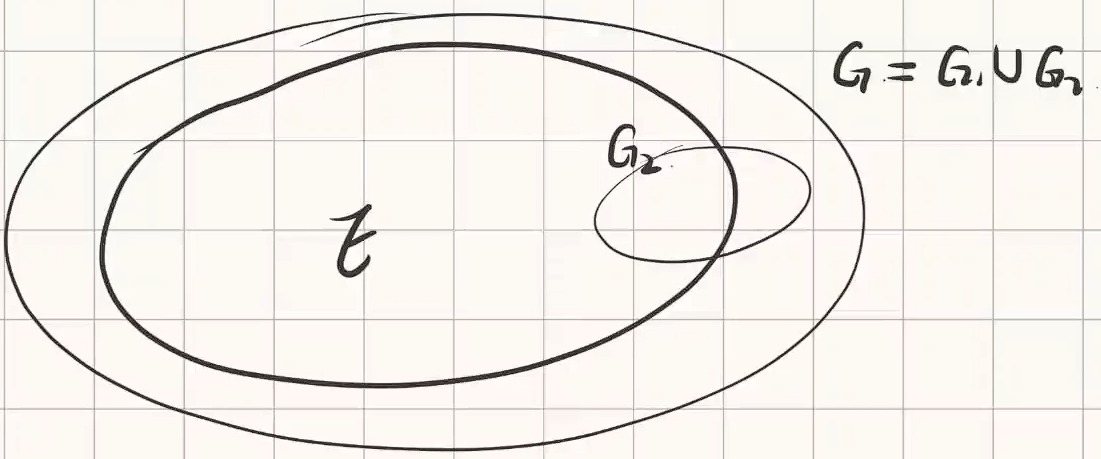
\includegraphics[width=0.5\linewidth]{figure/1.5-2}
				\caption{Prop \ref{prop 2.5.2}}
				\label{pic : prop 1.4.2} % 添加图像引用标签
			\end{figure}
		\end{proof}
	\end{enumerate}

\newpage

\subsection{$Cantor$集的性质}
	先来$Cantor$集的一些\textbf{刻画}.
	
	\vspace*{1em}
	\begin{itemize}
		\item $Cantor$集的直接定义:
		\begin{align}
			C = [0 , 1] \backslash \bigcup_{k = 0}^{\infty} \bigcup_{\substack{a_i \i \{ 0 , 2 \} \\ 1 \leq i \leq k}} \left( \sum_{j = 1}^{k}{\frac{a_j}{3^j}} + \frac{1}{3^{k + 1}} , \sum_{j = 1}^{k}{\frac{a_j}{3^j}} + \frac{2}{3^{k + 1}} \right)
		\end{align}
		
		\vspace*{6em}
		
		\item $Cantor$集的\textbf{三进制表示}:
		\begin{align}
			x \in C \,\, \Leftrightarrow \,\, x \,\, has \,\, a \,\, representation \,\, x = \sum_{k = 1}^{\infty}{a_k 3^{-k}} , \,\, a_k = 0 \,\, or \,\, 2
		\end{align}
		即
		\begin{align}
			C = \left\{ \sum_{k = 1}^{\infty}{a_k 3^{-k}} \mid a_k = 0 \,\, or \,\, 2 , \,\, k = 1 , 2 , \cdots \right\}
		\end{align}
	
		\begin{rmk}
			此处我们约定,若$x \in C$ 同时还存在有限表示形式,则我们取其\textbf{无穷表示}作为其\textbf{三进制表示}.
		\end{rmk}
	
		\begin{figure}[thbp!]
			\centering
			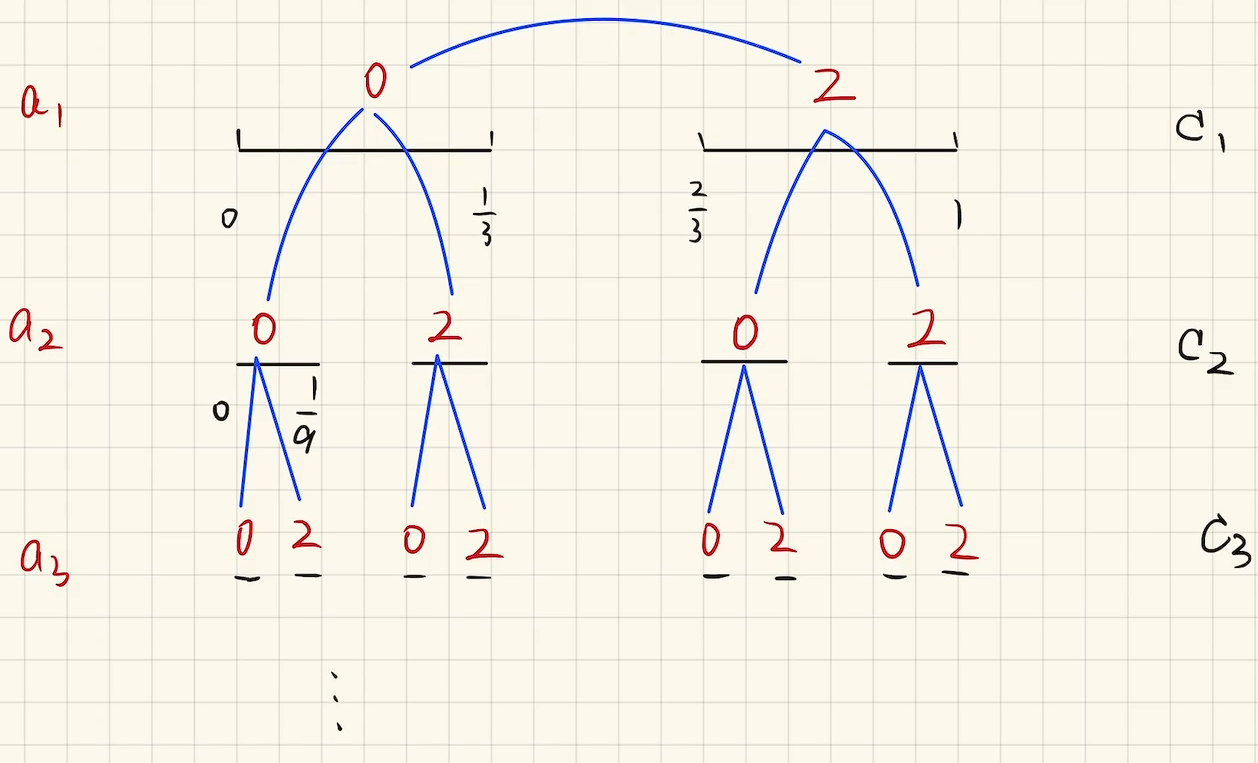
\includegraphics[width=0.7\linewidth]{figure/Cantor-1}
			\caption{$Cantor$集的\textbf{三进制表示}}
			\label{pic : Cantor} % 添加图像引用标签
		\end{figure}
	\end{itemize}
	
	\newpage
	
	\begin{enumerate}
		\item[4.] \textbf{Prop \ref{prop 2.5.3}. Cantor集的性质}. \\
		\begin{proof}
			\begin{enumerate}
				\item 
				\begin{enumerate}
					\item[(1)] $C$ is compact. \\
					Since $C \subset [0 , 1]$ is bounded and
					\begin{align}
						C = [0 , 1] \backslash \bigcup_{k = 0}^{\infty} \bigcup_{\substack{a_i \i \{ 0 , 2 \} \\ 1 \leq i \leq k}} \left( \sum_{j = 1}^{k}{\frac{a_j}{3^j}} + \frac{1}{3^{k + 1}} , \sum_{j = 1}^{k}{\frac{a_j}{3^j}} + \frac{2}{3^{k + 1}} \right) \,\, closed
					\end{align}
					Then $C \subset \R$ is bounded and closed, i.e. compact.
					
					\vspace*{8em}
					
					\item[(2)] $C$ is \textbf{nowhere dense} in $\R$. \\
					$\forall (\alpha , \beta) \subset \R$ open.
					\begin{enumerate}
						\item[$1^{\circ}$] If $(\alpha , \beta) \cap [0 , 1] = \varnothing$, then $(\alpha , \beta) \cap C = \varnothing$.
						
						\vspace*{2em}
						
						\item[$2^{\circ}$] If $(\alpha , \beta) \cap [0 , 1] \neq \varnothing$. Since
						\begin{align}
							C = [0 , 1] \backslash \bigcup_{k = 0}^{\infty} \bigcup_{\substack{a_i \i \{ 0 , 2 \} \\ 1 \leq i \leq k}} \left( \sum_{j = 1}^{k}{\frac{a_j}{3^j}} + \frac{1}{3^{k + 1}} , \sum_{j = 1}^{k}{\frac{a_j}{3^j}} + \frac{2}{3^{k + 1}} \right)
						\end{align}
						Then $\exists$ 充分大的$k_0$ 与适当的$a_j \in \{ 0 , 2 \} , \,\, j = 1 \sim k$, $\st$
						\begin{align}
							I_{n}^{k} = \left( \sum_{j = 1}^{k}{\frac{a_j}{3^j}} + \frac{1}{3^{k + 1}} , \sum_{j = 1}^{k}{\frac{a_j}{3^j}} + \frac{2}{3^{k + 1}} \right) \subset C^c \cap (\alpha , \beta) \subset (\alpha , \beta)
						\end{align}
						Let $(\alpha^{'} , \beta^{'}) = I_{n}^{k} \subset (\alpha , \beta)$. Then $(\alpha^{'} , \beta^{'}) \cap C = \varnothing$.
					\end{enumerate}
					
					\vspace*{2em}
					
					\begin{rmk}
						\textbf{Nowhere dense (无处稠密)}的定义如下:
						\begin{defn}\label{def a.5.1}
							在全集$X$ 中,$A \subset X$,若$(\overline{A})^{\circ} = \varnothing$,则称$A$ 在$X$ 中\underline{\textcolor{blue}{\textbf{无处稠密 (nowhere dense)}}}.
						\end{defn}
						更常使用其\textbf{等价定义}:
						\begin{align}
							&A \subset X \,\, nowhere \,\, dense \\
							&\Leftrightarrow \,\, \forall U \underset{open}{\subset} X , \,\, \exists O \subset U \,\, open , \,\, \st \,\, O \cap A = \varnothing
						\end{align}
						即对于$X$ 中任一开集$U$,都存在一个开子集$O$,使得$O$ 与$A$ 交集为空集.
					\end{rmk}
					
					\item[(3)] $C$ is \textbf{totally disconnected}. (\textbf{连通子集只有单点集},在$\R$ 中即等价于不存在区间) \\
					$\forall x , y \in C$, $x \neq y$, then $\exists \epsilon > 0$, $\st$
					\begin{align}
						\left| x - y \right| \geq \epsilon > 0
					\end{align}
					记$C_0 = [0 , 1]$, $C_k$ 表示经过$k$ 次操作后剩下的集合,则$C_0 \supset C_1 \supset \cdots$, $C = \overset{\infty}{\underset{k = 0}{\bigcap}}{C_k}$, $C_k$ 中每个连通分支的长度为$\frac{1}{3^k}$. \\
					For $\epsilon > 0$, $\exists n \in \N$, $\st$
					\begin{align}
						\frac{1}{3^n} < \epsilon
					\end{align}
					由于$x , y \in C = \overset{\infty}{\underset{k = 0}{\bigcap}}{C_k}$, 因此$x , y \in C_n$. 而$\left| x - y \right| \geq \epsilon > \frac{1}{3^n}$
					\begin{align}
						&\Rightarrow \,\, \text{$x$ 与$y$ 不在$C_n$ 同一道路分支中} \\
						&\Rightarrow \,\, \text{不妨设$x < y$, 则$\exists x < z < y$, $\st z \notin C$.}
					\end{align}
					\begin{center}
						(否则若$\forall z \in (x , y)$, $z \in C_n$, 则$[x , y] \subset C_n$, $x , y$ 属于$C_n$ 同一道路分支. 矛盾)
					\end{center}
					Therefore, $\forall x, y \in C$, $x < y$, $\exists x < z < y$, $\st z \notin C$. \\
					$\Rightarrow \,\, C$ is totally disconnected.
					
					\vspace*{4em}
					
					\begin{figure}[thbp!]
						\centering
						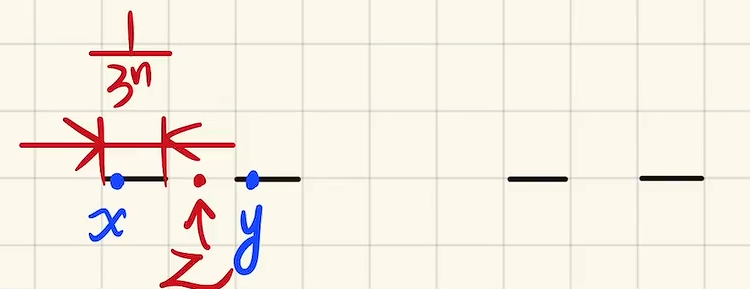
\includegraphics[width=0.6\linewidth]{figure/Cantor-2}
						\caption{$C$ totally disconnected}
						\label{pic : Cantor-2} % 添加图像引用标签
					\end{figure}
				
					\newpage
					
					\item[(4)] $C$ has no isolated points. ($C$ is \textbf{perfect}, i.e. closed + no isolated points) \\
					Suppose $x \in C = \overset{\infty}{\underset{k = 0}{\bigcap}}{C_k}$, $x \in C_k$, $\forall k$. \\
					In particular, for $n \in \N$, $x \in C_n$ \\
					$\Rightarrow \,\, x$ 落在$C_n$ 的某个连通分支中,即某个闭区间中. 记其一个区间端点为$y_n$. \\
					则不难证明,$y_n \in C = \overset{\infty}{\underset{k = 0}{\bigcap}}{C_k}$, and
					\begin{align}
						\left| x - y_n \right| \leq \frac{1}{3^n}
					\end{align}
					$\Rightarrow$ we get a sequence $\left\{ y_n \right\}_{n = 1}^{\infty}$, $y_n \rightarrow x$, $y_n \in C$, $\forall n$. \\
					$\Rightarrow \,\, x$ is not isolated. \\
					$\Rightarrow \,\, C$ is perfect.
				\end{enumerate}
			\end{enumerate}
		\end{proof}
	\end{enumerate}

\newpage
\section{$\S 2.1$}
	\begin{enumerate}
		\item \textbf{Thm \ref{thm 3.1.5}. 测度的完备性与几乎处处意义下可测性的传递}. \\
		\begin{proof}
			\begin{enumerate}
				\item [a.] \textbf{测度完备性与几乎处处相等意义下可测性的传递}. \\
				\begin{itemize}
					\item 必要性$\Rightarrow$: 记
					\begin{align}
						A = \left\{ x \in X \mid f(x) \neq g(x) \right\}
					\end{align}
					Then $\mu(A) = 0$. Thus
					\begin{align}
						g^{-1}((a , \infty]) = (g^{-1}((a , \infty]) \cap A) \bigsqcup (g^{-1}((a , \infty]) \cap A^c)
					\end{align}
					Since $\mu$ is complete and $f = g \,\, \mu$-a.e., then
					\begin{align}
						g^{-1}((a , \infty]) \cap A &\in \mathcal{M} \\
						g^{-1}((a , \infty]) \cap A^c = f^{-1}((a , \infty]) \cap A^c &\in \mathcal{M}
					\end{align}
					Therefore, $g^{-1}((a , \infty]) \in \mathcal{M} , \,\, \forall a \in \R$, $g$ is measurable.
					
					\vspace*{6em}
					
					\item 充分性$\Leftarrow$: Suppose $N \in \mathcal{M}$, $\mu(N) = 0$. $\forall F \subset N$, WTS: $F \in \mathcal{M}$. \\
					Suppose $f : X \rightarrow \overline{\R}$, $R(f) \subset [\alpha , \beta]$, where $0 < \alpha \leq \beta$. \\
					Let $g : X \rightarrow \overline{\R}$, $f \neq g$ only on $N$, with
					\begin{align}
						g|_{N} = (c \cdot \chi_{F})|_{N} , \,\, c > \beta
					\end{align}
					Then $f = g \,\, \mu$-a.e., $g$ is measurable. Therefore, $\forall d \in (\beta , c)$,
					\begin{align}
						g^{-1}((d , \infty]) = F \in \mathcal{M}
					\end{align}
					$\Rightarrow \,\, \mu$ is complete.
				\end{itemize}
				
				\newpage
				
				\item[b.] \textbf{测度完备性与几乎处处收敛意义下可测性的传递}. \\
				\begin{itemize}
					\item 必要性$\Rightarrow$: 记
					\begin{align}
						A = \left\{ x \in X \mid f_{n}(x) \not\to f(x) \right\}
					\end{align}
					Then $\mu(A) = 0$. Since $\mu$ is complete and $f_n$ is measurable, then \\
					$\Rightarrow \,\, f_{n}|_{A^c}$ is $\mathcal{M}_{A^c}$-measurable, and $f_{n}|_{A^c} \to f|_{A^c}$. \\
					$\Rightarrow \,\, f|_{A^c}$ is $\mathcal{M}_{A^c}$-measurable. \\
					$\Rightarrow \,\, f$ is measurable.
					
					\vspace*{12em}
					
					\item 充分性$\Leftarrow$: Suppose $N \in \mathcal{M}$, $\mu(N) = 0$. $\forall F \subset N$, WTS: $F \in \mathcal{M}$. \\
					Suppose $f_n : X \rightarrow \overline{\R}$ measurable and $R(f_n) \subset [\alpha , \beta]$, where $0 < \alpha \leq \beta$. \\
					Let $f : X \rightarrow \overline{\R}$, $f \neq f_n$ only on $N$, with
					\begin{align}
						f|_{N} = (c \cdot \chi_{F})|_{N} , \,\, c > \beta
					\end{align}
					Then $f_n \to f \,\, \mu$-a.e., $f$ is measurable. Therefore, $\forall d \in (\beta , c)$, 
					\begin{align}
						f^{-1}((d , \infty]) = F \in \mathcal{M}
					\end{align}
					$\Rightarrow \,\, \mu$ is complete.
				\end{itemize}
			\end{enumerate}
		\end{proof}
	\end{enumerate}
	

	%  ############################
	\ifx\allfiles\undefined
\end{document}
\fi